\chapter{Results and Discussion}
\label{chap:results}
    \section{OOV model}
        % \begin{figure}
        %   \centering
        %   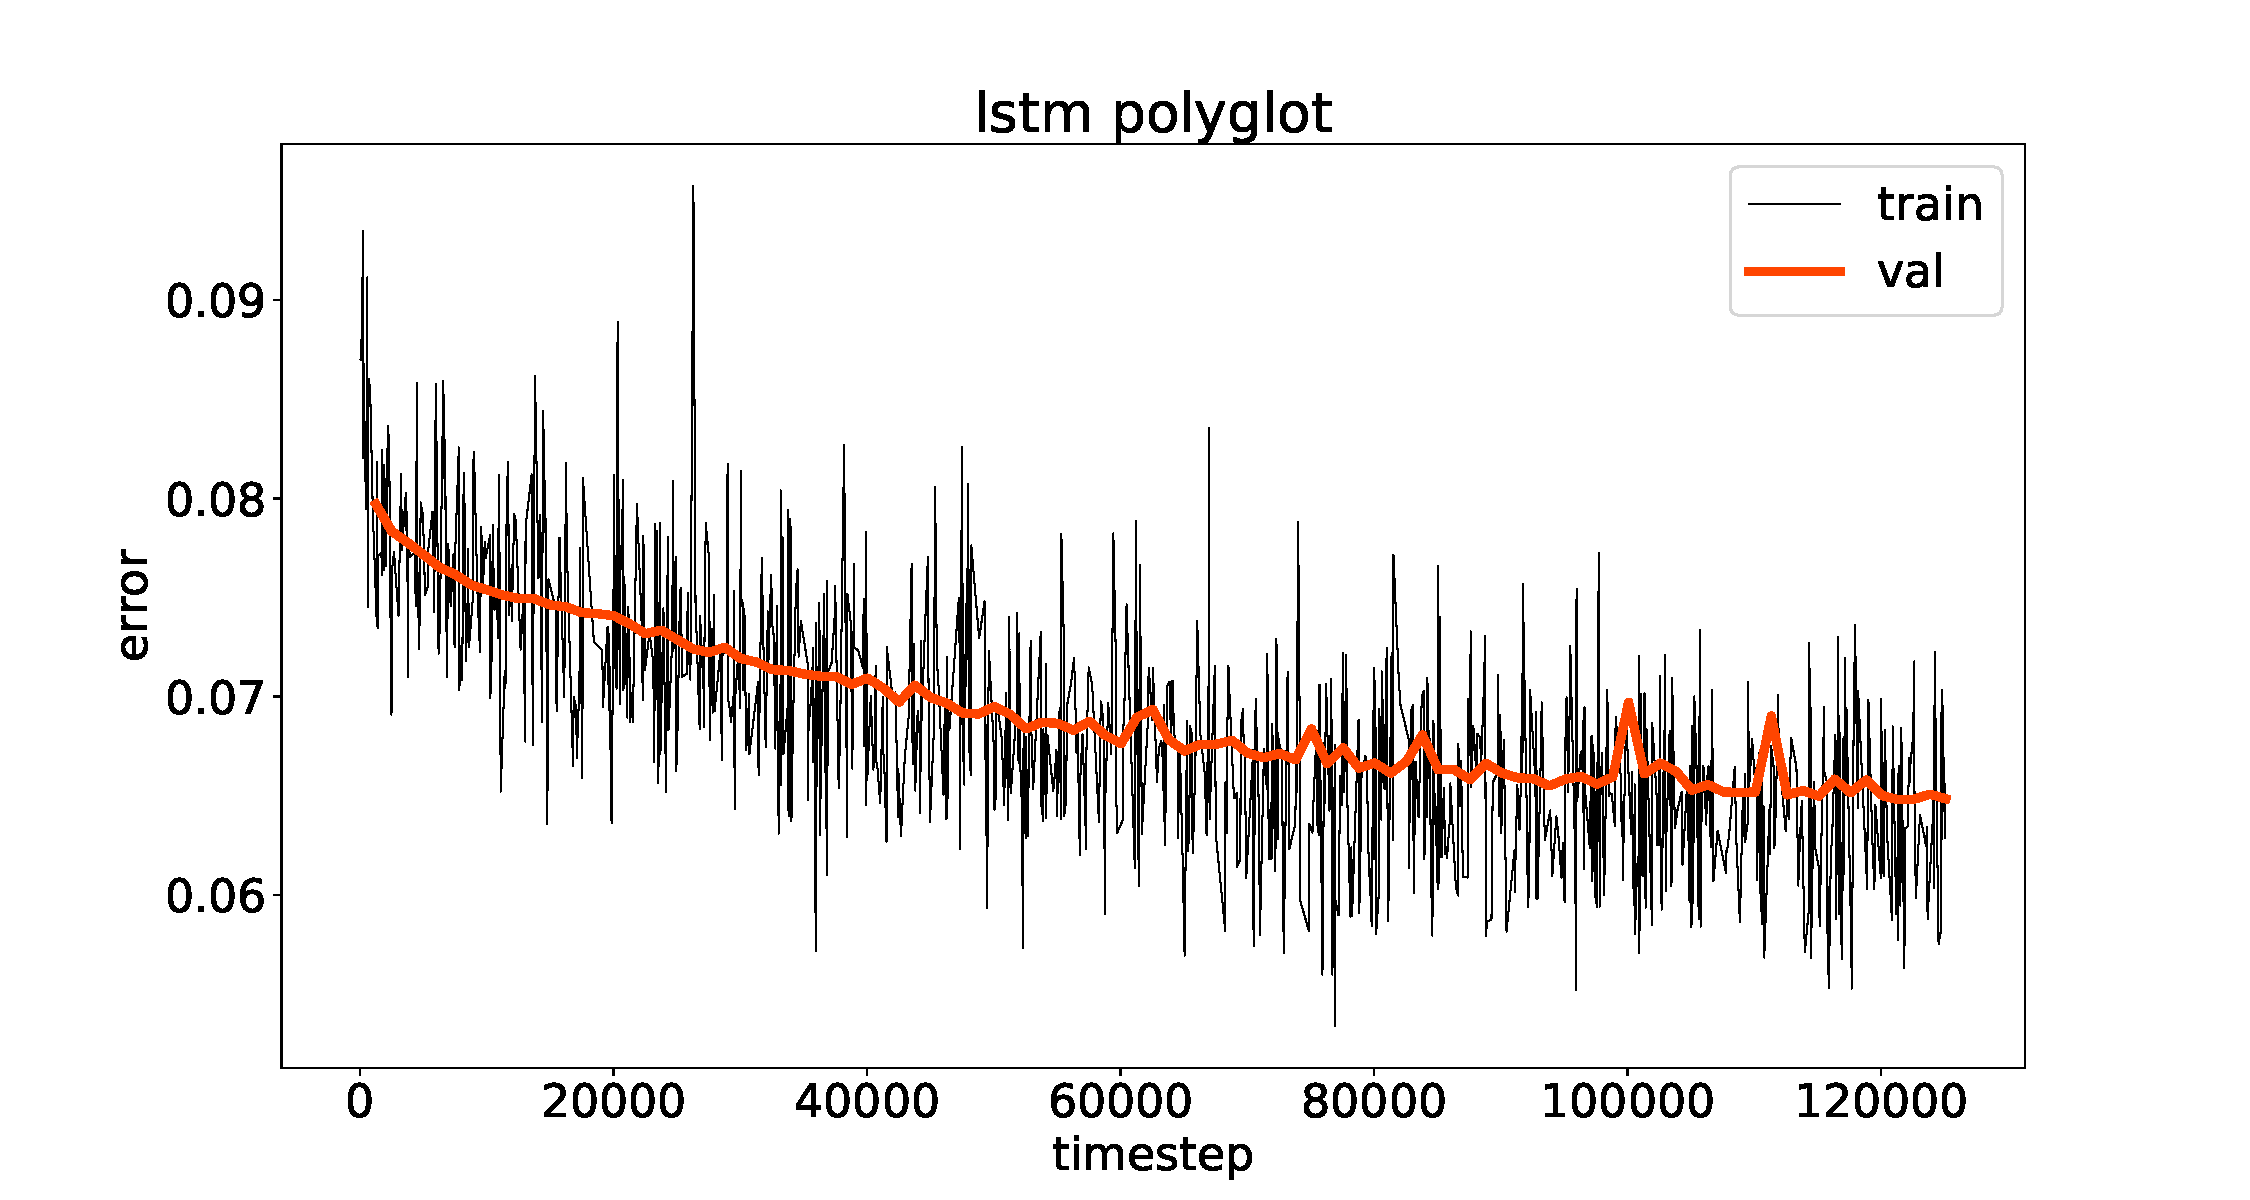
\includegraphics[width=.8\linewidth]{images/graph-lstm-polyglot.pdf}
        %   \caption{Train-val graph Mimick with polyglot}
        %   \label{fig:graph-lstm-polyglot}
        % \end{figure}
        % \begin{figure}
        %   \centering
        %   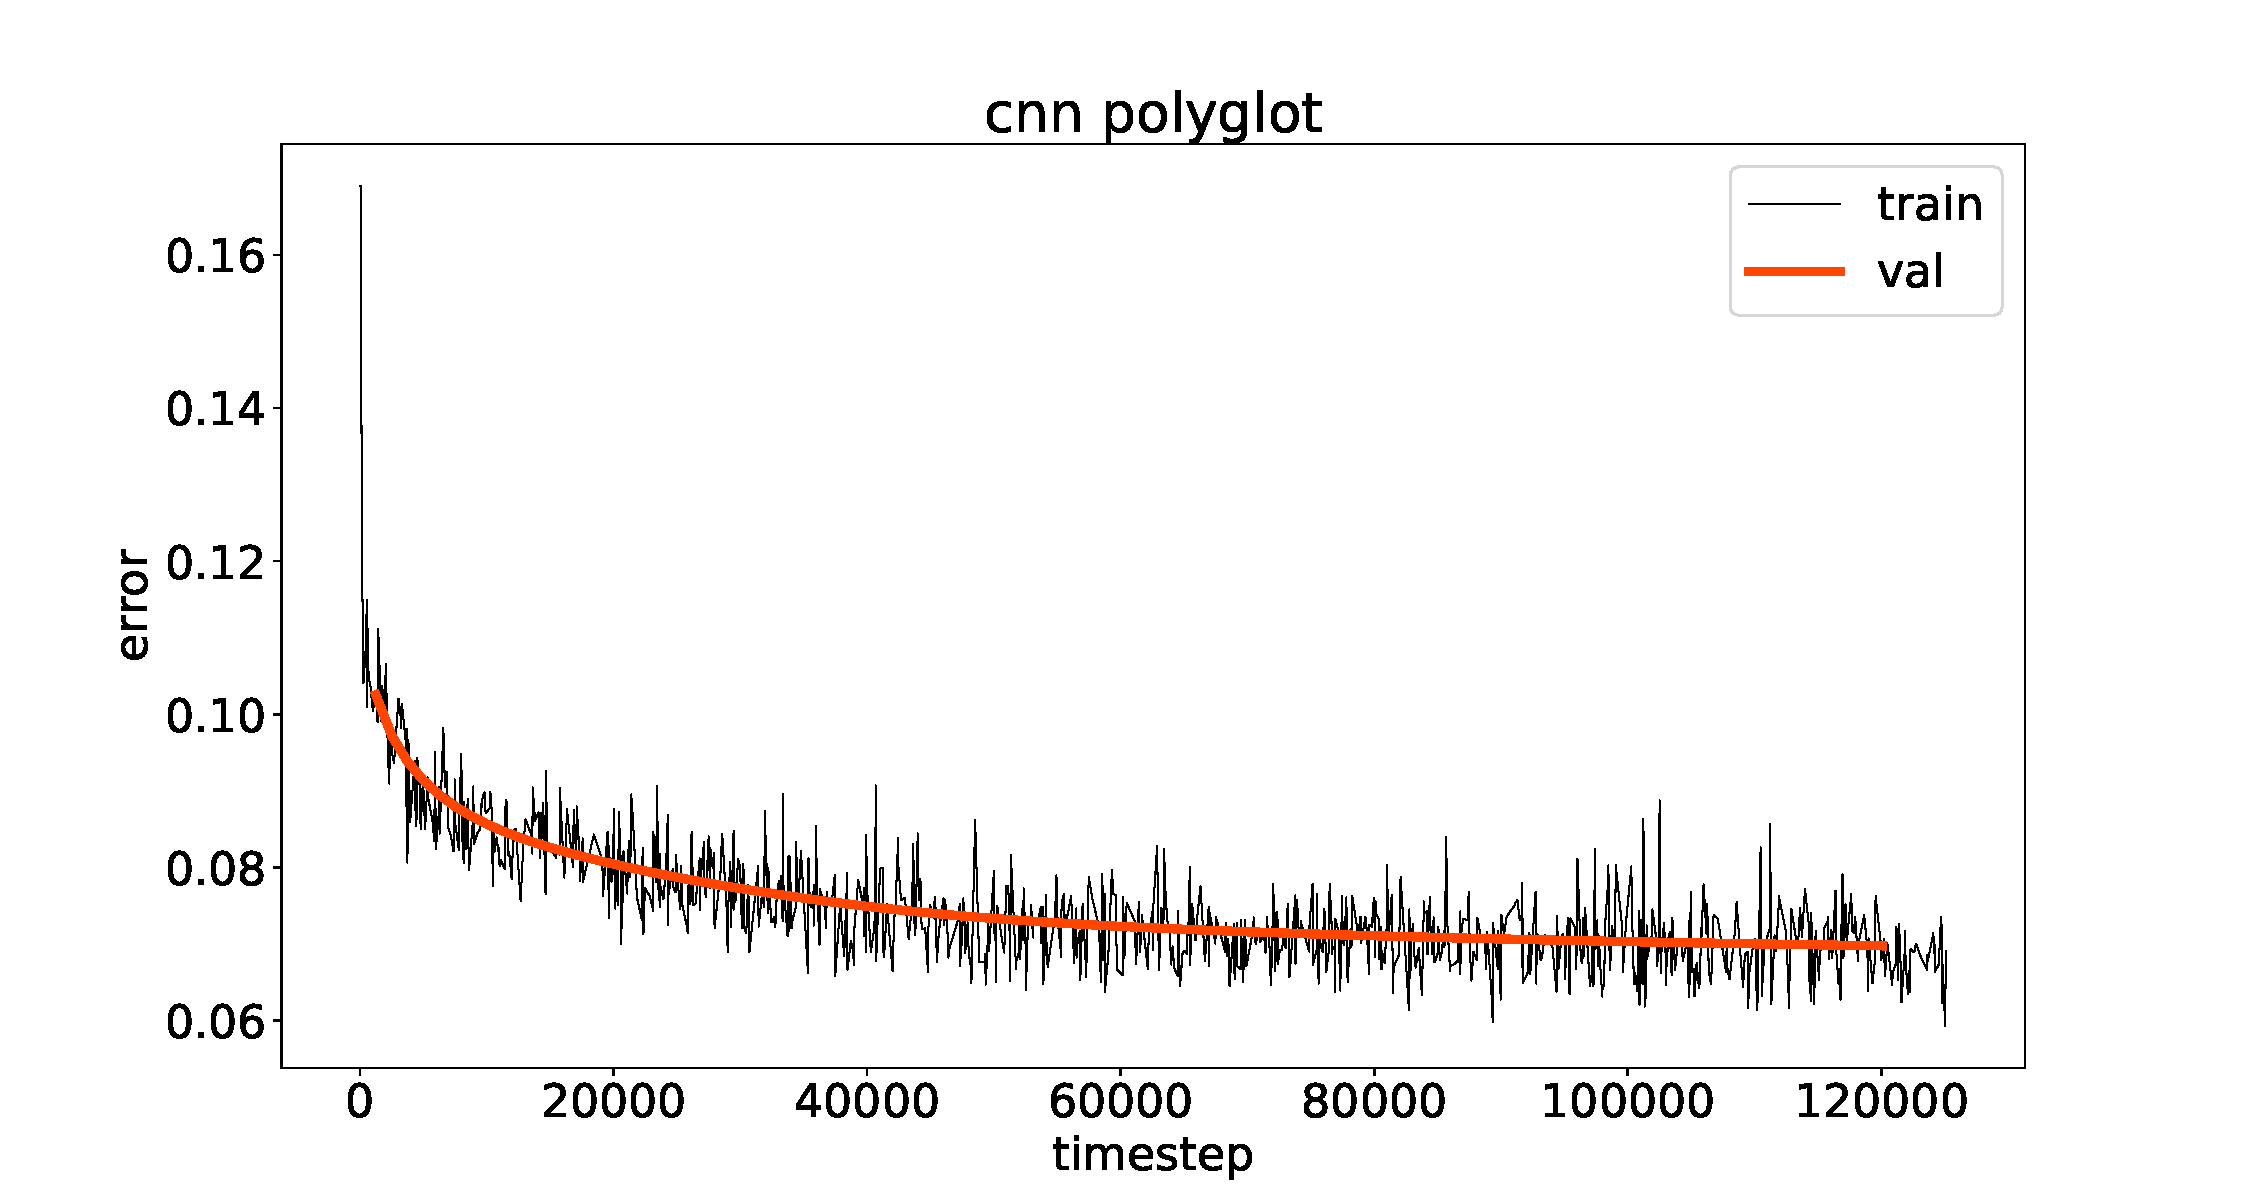
\includegraphics[width=.8\linewidth]{images/graph-cnn-polyglot.pdf}
        %   \caption{Train-val graph CNN with polyglot}
        %   \label{fig:graph-cnn-polyglot}
        % \end{figure}
        % \begin{figure}
        %   \centering
        %   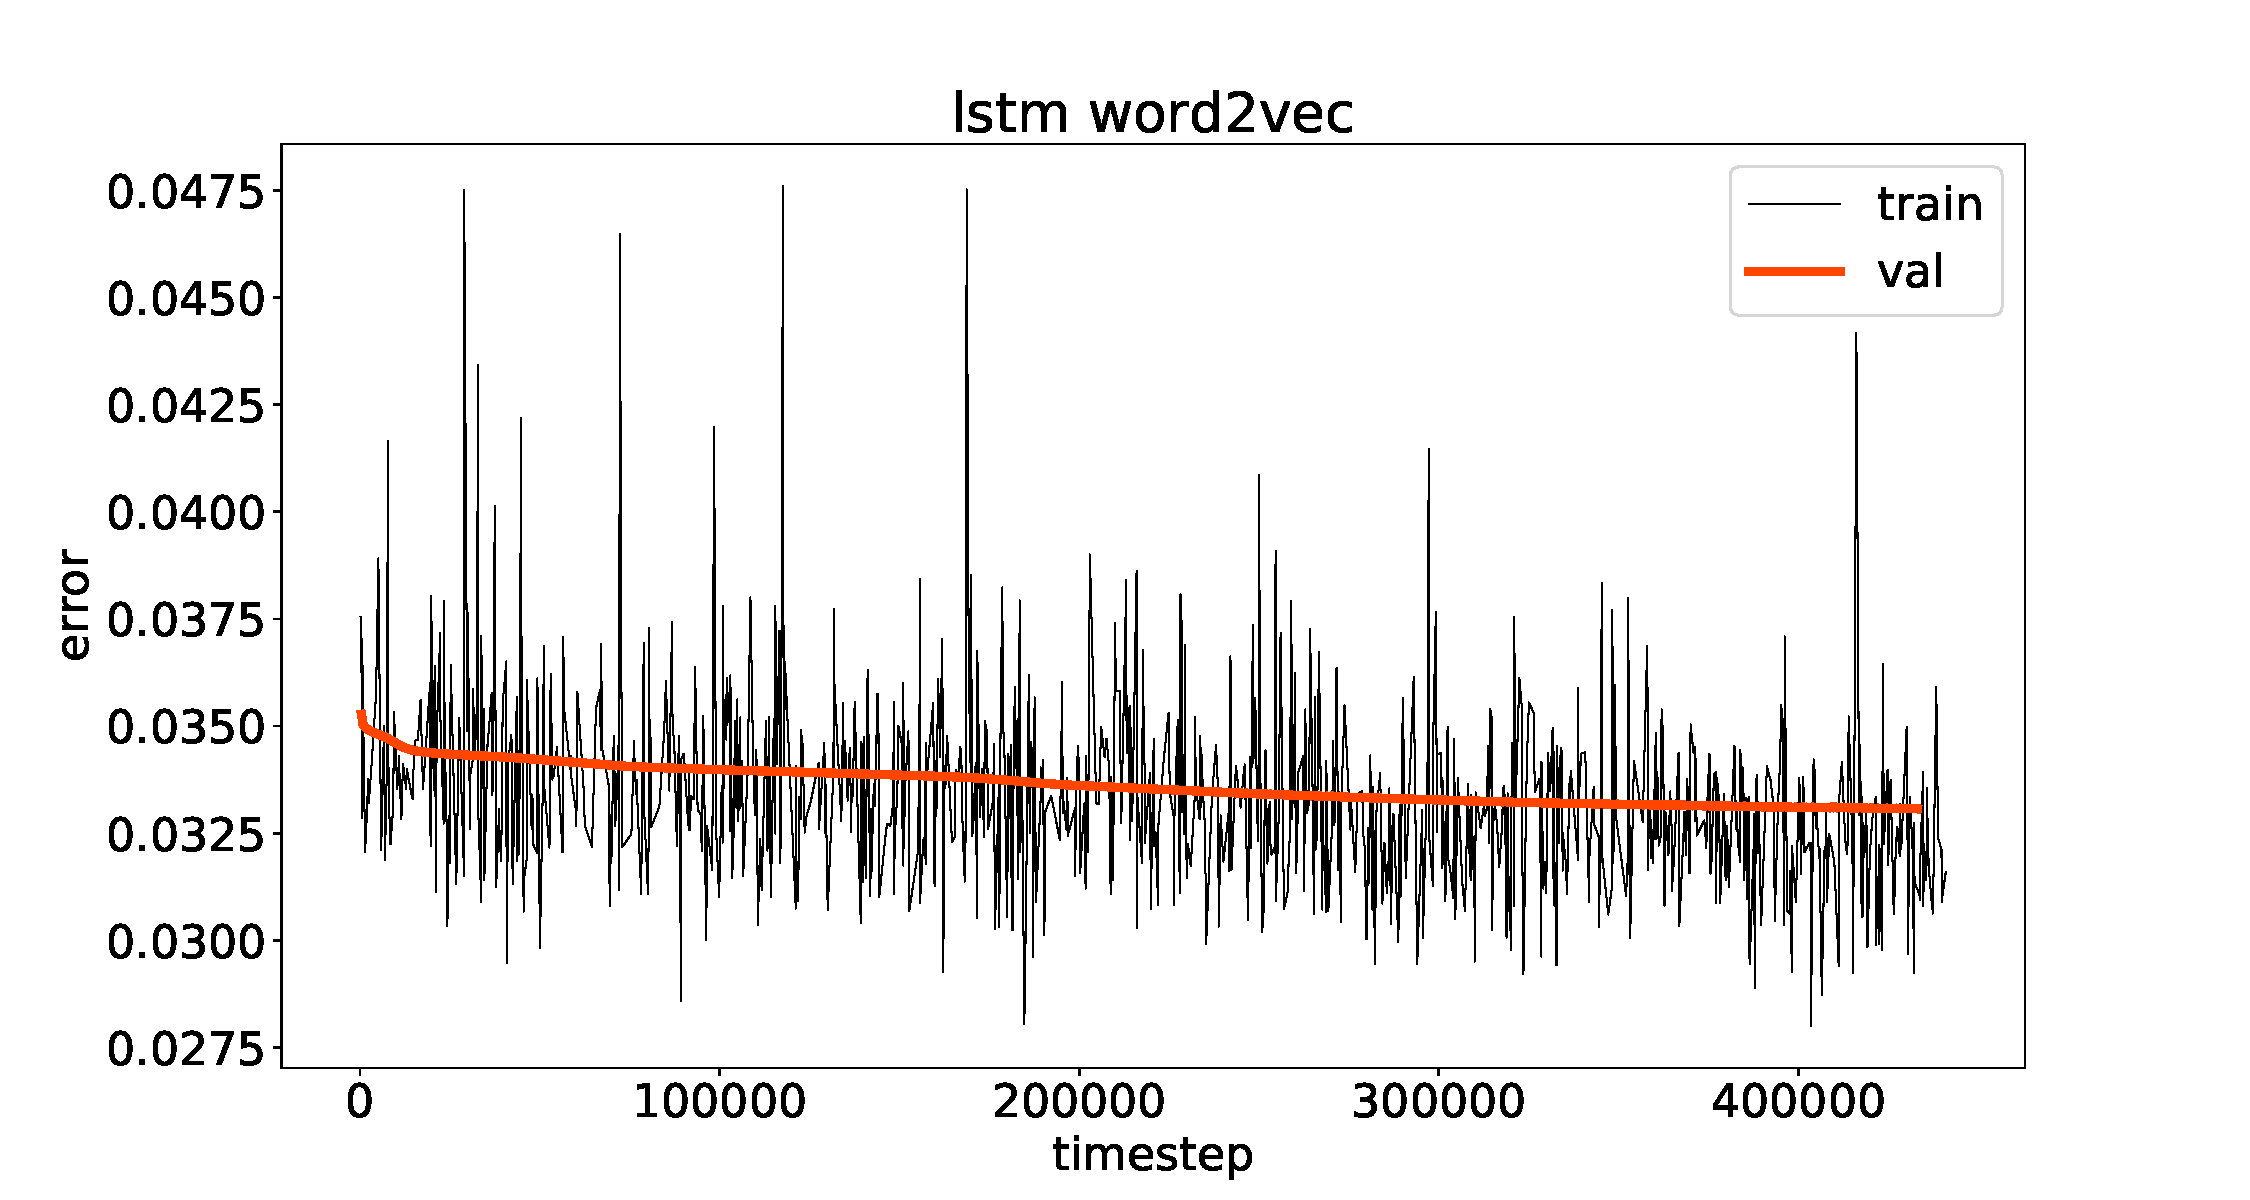
\includegraphics[width=.8\linewidth]{images/graph-lstm-word2vec.pdf}
        %   \caption{Train-val graph Mimick with word2vec}
        %   \label{fig:graph-lstm-word2vec}
        % \end{figure}
        % \begin{figure}
        %   \centering
        %   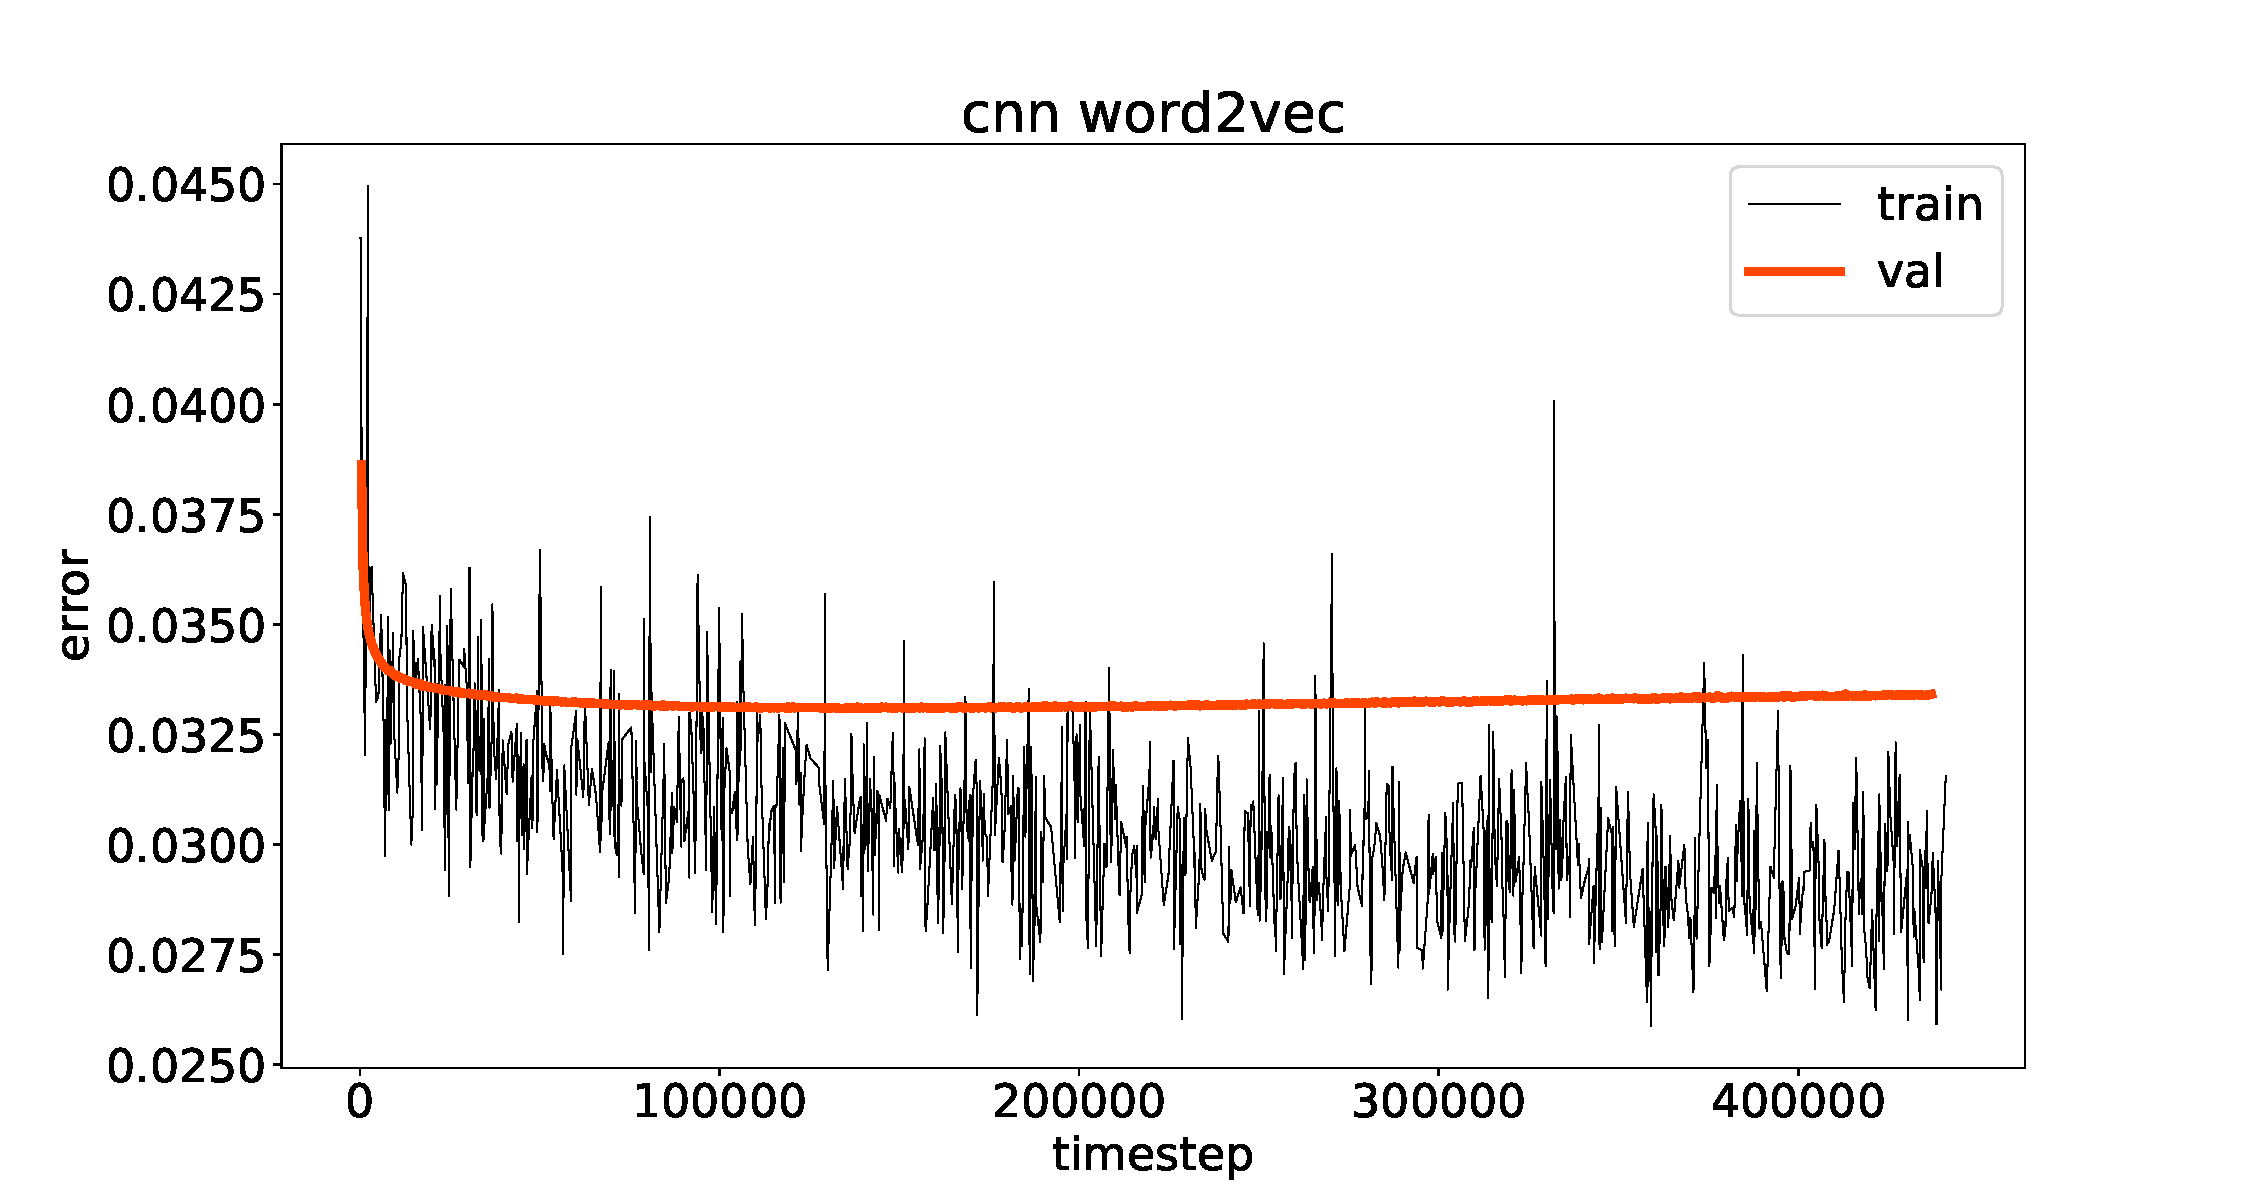
\includegraphics[width=.8\linewidth]{images/graph-cnn-word2vec.pdf}
        %   \caption{Train-val graph CNN with word2vec}
        %   \label{fig:graph-cnn-word2vec}
        % \end{figure}
        After training the model was done, some words were fed into
        the model and the nearest words appears in the vocabulary were
        calculated and shown on the table below. The input used are
        similar to the one used in testing \textsc{Mimick} on its
        original paper, though it might be hard to see the correlation
        between the input and the nearest neighbors since it is highly
        dependant on the vocabulary or pretrained embedding and the
        vocabulary size used for training, thus reliance on dictionary
        and search engine were needed although it is not scientific.

        Both model CNN and \textsc{Mimick} results that were trained
        with word2vec are shown on Table
        \ref{tab:nearest:cnn-word2vec} and Table
        \ref{tab:nearest:lstm-word2vec} respectively. The first test
        word were an abbreviation "MCT" with length of three
        characters and all-capitalize. Both model were able to predict
        that the nearest neighbors are also another abbreviation. For
        name as input, "McNeally" and "Vercelloti", both model were
        able to predict the nearest neighbor to be name as well, as
        shown on Table \ref{tab:nearest:cnn-word2vec} and Table
        \ref{tab:nearest:lstm-word2vec}. For "McNeally" the nearest
        neighbor were English name for male for both models.
        Interestingly for "Vercellotti", \textsc{Mimick} predicted
        that the nearest neighbor was former American baseball player,
        while CNN predicted that the nearest neighbor was Ukrainian
        politician. For an adjective input "Secretive", both model
        were predicted that the nearest neighbors are group of verbs,
        nouns, adjectives, and adverbs. Both models were also able to
        handle typography error like "corssing" and "developiong",
        only that CNN model nearest word were "developing" while
        \textsc{Mimick} were a verb that has suffix \textit{-ing}. The
        nearest neighbors for corssing were also verb with suffix
        \textit{-ing}. Interestingly, for both model, nearest neighbor
        for flatfish has no correlation at all.

        Similar nearest neighbors were also produced by the model when
        trained with polyglot \citep{polyglot2013alrfou} only with
        different set of words for each input.

        \begin{table}[H]
          \begin{center}
            \caption{Nearest Neighbors Mimick (word2vec)}
            ~\\
            \label{tab:nearest:lstm-word2vec}
            \begin{tabular}{c|l}
              \textbf{Word} & \textbf{Nearest Neighbors}\\
              \hline
              MCT & EC ATI BT SMC Nvidia\\
              McNeally & Miller Smith McKee Grimes Thompson\\
              Vercellotti & Smoltz Pettitte Pujols Buehrle Peavy\\
              Secretive & Seeks Approves Expands Implementation Preview\\
              corssing & turning talking putting squeezing shifting\\
              flatfish & just sort anyway things silly\\
              compartmentalize & subjective appropriate constrained decentralized regard\\
              pesky & just anyway maybe guess something\\
              lawnmower & it liberalism something anyway kind\\
              developiong & undermining implementing reshaping diminishing destroying\\
              hurtling & squeezing ripping turning pulling chasing\\
              expectedly & undermined unaware understood exposed utilized\\
            \end{tabular}
          \end{center}
        \end{table}

        \begin{table}[H]
          \begin{center}
            \caption{Nearest Neighbors CNN (word2vec)}
            ~\\
            \label{tab:nearest:cnn-word2vec}
            \begin{tabular}{c|l}
              \textbf{Word} & \textbf{Nearest Neighbors}\\
              \hline
              MCT & DPP PCT PMC TSMC RTA\\
              McNeally & Murphy McCullough McIntyre Gallagher Delaney\\
              Vercellotti & Yanukovych Tymoshenko Yushchenko Saakashvili Ancelotti\\
              Secretive & Important Acquisition Process Benefits Transactions\\
              corssing & putting turning squeezing pulling sneaking\\
              flatfish & Wasps Premiership footballing Saracens flavorful\\
              compartmentalize & efficiencies retrofit development commercialize integrate\\
              pesky & weird cranky goofy scary joked\\
              lawnmower & driveway sidewalk porch mother creek\\
              developiong & developing development develop reshaping investment\\
              hurtling & knocking chasing tearing ripping slamming\\
              expectedly & predictably certainly unbelievably amazingly quite\\
            \end{tabular}
          \end{center}
        \end{table}

        
        
        \begin{table}[!ht]
          \begin{center}
            \caption{Nearest Neighbors Mimick (polyglot)}
            ~\\
            \label{tab:nearest:lstm-polyglot}
            \begin{tabular}{c|l}
              \textbf{Word} & \textbf{Nearest Neighbors}\\
              \hline
              MCT & \multicolumn{1}{p{0.7\textwidth}}{NAL MIB AWS SIA SMP}\\
              McNeally & \multicolumn{1}{p{0.7\textwidth}}{McCready Hiatt Tolan McAdams Coxon}\\
              Vercellotti & \multicolumn{1}{p{0.7\textwidth}}{Aurich Cavour Gubbio Barcelos Camoes}\\
              Secretive & \multicolumn{1}{p{0.7\textwidth}}{Rhetorical Predictive Contextual Affective Perceptual}\\
              corssing & \multicolumn{1}{p{0.7\textwidth}}{inflating straining concealing compromising channeling}\\
              flatfish & \multicolumn{1}{p{0.7\textwidth}}{whirlpool cocoon diaper crevice gutter}\\
              compartmentalize & \multicolumn{1}{p{0.7\textwidth}}{reproducible quantifiable repeatable synergistic biologic}\\
              pesky & \multicolumn{1}{p{0.7\textwidth}}{waxy lozenge phosphor thermoplastic flake}\\
              lawnmower & \multicolumn{1}{p{0.7\textwidth}}{dishwasher caddy welder motorist rowboat}\\
              developiong & \multicolumn{1}{p{0.7\textwidth}}{compromising inflating loosening halting venting}\\
              hurtling & \multicolumn{1}{p{0.7\textwidth}}{splashing blasting shredding combing pounding}\\
              expectedly & \multicolumn{1}{p{0.7\textwidth}}{realistically energetically conspicuously materially imperfectly}\\
            \end{tabular}
          \end{center}
        \end{table}

        \begin{table}[!ht]
          \begin{center}
            \caption{Nearest Neighbors CNN (polyglot)}
            ~\\
            \label{tab:nearest:cnn-polyglot}
            \begin{tabular}{c|l}
              \textbf{Word} & \textbf{Nearest Neighbors}\\
              \hline
              MCT & \multicolumn{1}{p{0.7\textwidth}}{NDS TEN GTC CPO UNI}\\
              McNeally & \multicolumn{1}{p{0.7\textwidth}}{briefly quietly Akerman enthusiastically Coons}\\
              Vercellotti & \multicolumn{1}{p{0.7\textwidth}}{Hassel Lemaire Sarno Perrot Necker}\\
              Secretive & \multicolumn{1}{p{0.7\textwidth}}{Rhetorical Subjective Legitimate Contextual Constructive}\\
              corssing & \multicolumn{1}{p{0.7\textwidth}}{confining straining inflating impacting shrinking}\\
              flatfish & \multicolumn{1}{p{0.7\textwidth}}{narcotic transient hangover lameness stench}\\
              compartmentalize & \multicolumn{1}{p{0.7\textwidth}}{commercialisation numeracy alertness institutionalization practicality}\\
              pesky & \multicolumn{1}{p{0.7\textwidth}}{eyeballs jerky wrinkles fuss bruise}\\
              lawnmower & \multicolumn{1}{p{0.7\textwidth}}{lavatory washroom toilet restroom mattress}\\
              developiong & \multicolumn{1}{p{0.7\textwidth}}{distancing compromising orienting manoeuvring harmonizing}\\
              hurtling & \multicolumn{1}{p{0.7\textwidth}}{compromising confining inflating lightening channeling}\\
              expectedly & \multicolumn{1}{p{0.7\textwidth}}{substantively realistically sensibly procedurally irrevocably}\\
            \end{tabular}
          \end{center}
        \end{table}


    \section{POStagging results}
      \begin{figure}[H]
        \centering
        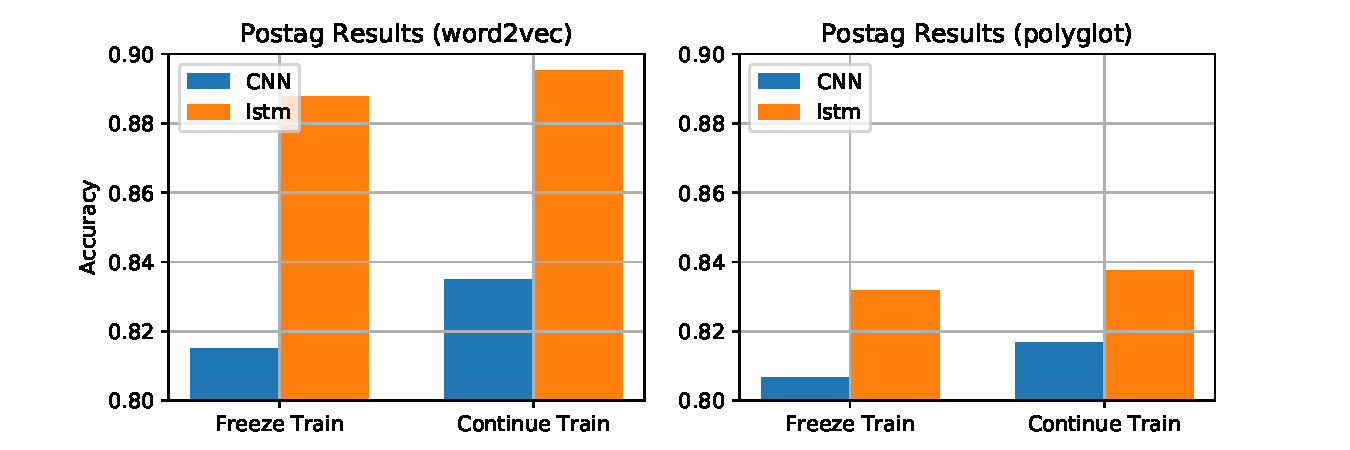
\includegraphics[width=\linewidth]{images/postag_results.pdf}
        \caption{POStagging results}
        \label{fig:postag_results}
      \end{figure}
      The OOV embedding from both model on top of the pretrained
      embedding were used as input for POStagging task. Firstly, the
      OOV model were frozen, meaning that the OOV model output were
      used as input as is by setting the weight to be frozen.
      Secondly, the OOV model were also trained in conjunction with
      the POStagger to improve accuracies of the POStagger. The
      improvement on both models and both pretrained embedding by
      allowing the OOV model to be trained during training the
      POStagger can be seen on Figure \ref{fig:postag_results}.

      Both frozen training and continued training for CNN model has
      higher accuracies compared to \textsc{Mimick}. It shows that CNN
      model are better to handle POStagging than \textsc{Mimick}.

    \section{Word Similarity}
    % \begin{table}[h!]
    %   \begin{center}
    %     \caption{Word Similarity Task Results}
    %     ~\\
    %     \label{tab:table1}
    %     \begin{tabular}{l|c|c|c|c|c|c|c|c|}
    %       ~ & \multicolumn{4}{c|}{\textbf{word2vec}} & \multicolumn{2}{c|}{\textbf{polyglot}} & \multicolumn{2}{c|}{\textbf{dict2vec}}\\
    %       \hline
    %       \textbf{Dataset} & \textbf{OOV} & \textbf{invocab} &
    %       \textbf{CNN} & \textbf{Mimick} &
    %       \textbf{CNN} & \textbf{Mimick} &
    %       \textbf{CNN} & \textbf{Mimick}\\
    %       \hline
    %       card & 989 & 317 & 71.39 & 85.65\\
    %       mc30 & 4 & 35 & 714.29 & 731.64\\
    %       men & 82 & 669 & 681.98 & 668.05\\
    %       mturk287 & 95 & 404 & 605.97 & 542.96\\
    %       mturk771 & 17 & 1096 & 656.73 & 654.57\\
    %       rg65 & 2 & 46 & 663.70 & 714.45\\
    %       rwstanford & 1488 & 1463 & 301.63 & 291.60\\
    %       simlex & 17 & 1011 & 429.11 & 429.57\\
    %       simverb & 90 & 737 & 308.92 & 310.88\\
    %       verb143 & 4 & 113 & 485.09 & 483.57\\
    %       wordsim & 13 & 424 & 647.94 & 648.74\\
    %       yp130 & 5 & 142 & 483.99 & 461.94\\
    %       \hline
    %       \multicolumn{3}{c|}{average} & 504.22 &
    %       501.97\\
    %     \end{tabular}
    %   \end{center}
    % \end{table}
    \begin{table}[!ht]
      \begin{threeparttable} 
      \begin{center}
        \caption{Word Similarity Task Results (word2vec)}
        ~\\
        \label{tab:wordsim:word2vec}
        \begin{tabular}{l|c|c|c|c|c}
          \textbf{Dataset} & \textbf{OOV} & \textbf{Invocab} & \textbf{OOV Ratio} & \textbf{CNN}\tnote{*} & \textbf{Mimick}\tnote{*}\\
          \hline
          card & 989 & 317 & 75.73\% & 71.39 & 85.65\\
          mc30 & 4 & 35 & 10.26\% & 714.29 & 731.64\\
          men & 82 & 669 & 10.92\% & 681.98 & 668.05\\
          mturk287 & 95 & 404 & 19.04\% & 605.97 & 542.96\\
          mturk771 & 17 & 1096 & 1.53\% & 656.73 & 654.57\\
          rg65 & 2 & 46 & 4.17\% & 663.70 & 714.45\\
          rwstanford & 1488 & 1463 & 50.42\% & 301.63 & 291.60\\
          simlex & 17 & 1011 & 1.65\% & 429.11 & 429.57\\
          simverb & 90 & 737 & 10.88\% & 308.92 & 310.88\\
          verb143 & 4 & 113 & 3.42\% & 485.09 & 483.57\\
          wordsim & 13 & 424 & 2.97\% & 647.94 & 648.74\\
          yp130 & 5 & 142 & 3.40\% & 483.99 & 461.94\\
          \hline
          \multicolumn{4}{r|}{\textbf{average}} & 504.23 & 501.97\\
        \end{tabular}
        \begin{tablenotes}
          \item[*] multiplied by 1000
        \end{tablenotes}
      \end{center}
      
    \end{threeparttable} 
    \end{table}

    On Table \ref{tab:wordsim:word2vec}, the model trained with
    word2vec \citep{Distributed2013mikolov}. The predicted embedding
    then used for calculating the spearman rank correlation. For
    easier reading, all the results of word similarity task shown in
    the table and the texts were multiplied by 1000. From 12 word
    similarity datasets, CNN model has higher Spearman correlation
    coefficient on 6 datasets with averaged Spearman correlation
    coefficient of $504.23$ compared to \textsc{Mimick} that achieved
    $501.97$.

    \begin{table}[!ht]
      \begin{threeparttable} 
      \begin{center}
        \caption{Word Similarity Task Results (polyglot)}
        ~\\
        \label{tab:wordsim:polyglot}
        \begin{tabular}{l|c|c|c|c|c}
          \textbf{Dataset} & \textbf{OOV} & \textbf{Invocab} & \textbf{OOV Ratio} & \textbf{CNN}\tnote{*} & \textbf{Mimick}\tnote{*}\\
          \hline
          card & 864 & 442 & 66.16\% & 125.61 & 78.16\\
          mc30 & 1 & 38 & 2.56\% & 595.91 & 580.77\\
          men & 14 & 737 & 1.86\% & 486.48 & 487.51\\
          mturk287 & 76 & 423 & 15.23\% & 457.89 & 443.08\\
          mturk771 & 3 & 1110 & 0.27\% & 432.90 & 432.99\\
          rg65 & 1 & 47 & 2.08\% & 530.47 & 525.82\\
          rwstanford & 999 & 1952 & 33.85\% & 298.92 & 260.79\\
          simlex & 4 & 1024 & 0.39\% & 234.81 & 234.86\\
          simverb & 53 & 774 & 6.41\% & 136.38 & 135.24\\
          verb143 & 0 & 117 & 0.00\% & 335.81 & 335.81\\
          wordsim & 0 & 437 & 0.00\% & 410.28 & 408.60\\
          yp130 & 5 & 142 & 3.40\% & 29.54 & 52.71\\
          \hline
          \multicolumn{4}{r|}{average} & 339.58 & 331.36\\
        \end{tabular}
        \begin{tablenotes}
          \item[*] multiplied by 1000
        \end{tablenotes}
      \end{center}
    \end{threeparttable} 
    \end{table}

    The same procedure for both models trained with polyglot
    \citep{polyglot2013alrfou}. From 12 word similarity datasets,
    \textsc{Mimick} only has 5 datasets that has higher Spearman
    correlation coefficient than CNN model. In contrast with the model
    trained with word2vec \citep{Distributed2013mikolov}, the model
    trained with polyglot \citep{polyglot2013alrfou} only achived
    Spearman correlation coefficient as high as $339.55$ and $331.30$
    for CNN and \textsc{Mimick} respectively as shown on Table
    \ref{tab:wordsim:polyglot}.

    \begin{table}[!ht]
      \begin{threeparttable} 
      \begin{center}
        \caption{Word Similarity Task Results (dict2vec)}
        ~\\
        \label{tab:wordsim:dict2vec}
        \begin{tabular}{l|c|c|c|c|c|c}
          \textbf{Dataset} & \textbf{OOV} & \textbf{Invocab} &
          \textbf{OOV Ratio} & \textbf{dict2vec}\tnote{*} &
          \textbf{CNN}\tnote{*} & \textbf{Mimick}\tnote{*}\\
          \hline
          card & 828 & 478 & 63.40\% & 48.07 & 112.75 & 74.61\\
          mc30 & 0 & 39 & 0.00\% & 847.57 & 847.57 & 847.57\\
          men & 1 & 750 & 0.13\% & 713.16 & 723.76 & 719.79\\
          mturk287 & 2 & 497 & 0.40\% & 652.27 & 651.04 & 652.05\\
          mturk771 & 0 & 1113 & 0.00\% & 683.91 & 683.91 & 683.91\\
          rg65 & 0 & 48 & 0.00\% & 832.86 & 832.86 & 832.86\\
          rwstanford & 619 & 2332 & 20.98\% & 214.60 & 424.97 & 426.77\\
          simlex & 3 & 1025 & 0.29\% & 454.80 & 457.11 & 458.45\\
          simverb & 24 & 803 & 2.90\% & 375.15 & 394.41 & 392.98\\
          verb143 & 0 & 117 & 0.00\% & 187.82 & 187.82 & 187.82\\
          wordsim & 18 & 419 & 4.12\% & 642.71 & 713.81 & 710.63\\
          yp130 & 2 & 145 & 1.36\% & 577.76 & 618.56 & 630.99\\
          \hline
          \multicolumn{4}{r|}{average} & 519.22 & 554.05 & 551.54\\
        \end{tabular}
        \begin{tablenotes}
          \item[*] multiplied by 1000
        \end{tablenotes}
      \end{center}
    \end{threeparttable} 
    \end{table}

    For baseline embedding dict2vec \citep{dict2vect2017tissier}. the
    original embedding added with random embedding for OOV handling
    were also compared with CNN and \textsc{Mimick} models. Dict2vec
    only able to achieve Spearman correlation coefficient of $519.22$.
    In contrast CNN model an \textsc{Mimick} model were able to
    achieve $554.05$ and $551.54$ on average respectively as shown on
    Table \ref{tab:wordsim:dict2vec}. This shows that both OOV models
    can handle OOV better than initializing embedding randomly for
    OOV. On top of that, from three pretrained embeddings, CNN model
    performs better than \textsc{Mimick} for word similarity task.